
%使用XeLaTeX编译
%版权所有,翻版必究
%本文件由程序自动生成,任何修改将被覆盖
%2019 年 01 月 23 日



%Gook Luck!

\FloatBarrier
\section{
qmake入门
}\label{s100310}


qmake类似于cmake,但qmake比cmake更加简洁清晰。
如果读者希望写一个跨平台的通用库的话,
或许cmake是比qmake更加优异的选择。
但读者明确是写一个特定的应用程序的话,
qmake就比cmake优秀的多。
qmake比cmake功能较少,
但从另一个角度,
qmake比cmake更加专注。
通过本节,
读者会发现只需要学习可怜的一点内容,
就可以使用qmake搭建出复杂的程序架构。
不过,本书毕竟是一门专门写Qt Quick的书,
不可能介绍qmake的每一个细节。

%%%%%%%%%%%%%%%%%%%%%%%%%%%%%%%%%%%%%%%%%%%%%%%%%%%%%%%%
\FloatBarrier
\subsection{
使用qmake构建Hellow World!
}\label{ss000610}

读者新建一个目录\footnote{
本书所有目录都要求不包含空格和中文,以后不再赘述。
},
在此文件夹下新建一个“hellow\underline{\hspace{0.5em}}world.pro”文件,输入文件内容如
\filesourcenumbernameone\ \ref{f000002}。
在此文件夹下建立“main.cpp”文件,输入内容如
\filesourcenumbernameone\ \ref{f000003}。

%\begin{spacing}{1.0}
\refstepcounter{filesourcenumber}\label{f000002}    %增加源代码编号
\FloatBarrier                                  %强制完成浮动体布局
\begin{thebookfilesourceone}[escapeinside={(*@}{@*)},
caption=GoodLuck,
title=\filesourcenumbernameone \thefilesourcenumber
]
QT -= gui
QT -= core

CONFIG += console

CONFIG(debug,debug|release){
    TARGET = hellow_word_debug
}else{
    TARGET = hellow_word
}

TEMPLATE = app

win32-msvc*{
    QMAKE_CXXFLAGS += /std:c++latest
}else{
    CONFIG += c++17
}

SOURCES += $$PWD/main.cpp
DESTDIR =  $$PWD

DEFINES *= NUMBER=1
DEFINES *= HELLOW=\\\"Hellow\\\"
DEFINES += QT_DEPRECATED_WARNINGS(*@\marginpar[\hfill\setlength\fboxsep{2pt}\fbox{\footnotesize{\kaishu\parbox{1em}{\setlength{\baselineskip}{2pt}\filesourcenumbernameone}}\footnotesize{\thefilesourcenumber}}]{\setlength\fboxsep{2pt}\fbox{\footnotesize{\kaishu\parbox{1em}{\setlength{\baselineskip}{2pt}\filesourcenumbernameone}}\footnotesize{\thefilesourcenumber}}}@*)\end{thebookfilesourceone}          %抄录环境
\addtocounter{lstlisting}{-1}   %sub lstlisting counter ...
%\end{spacing}

%\begin{spacing}{1.0}
\refstepcounter{filesourcenumber}\label{f000003}    %增加源代码编号
\FloatBarrier                                  %强制完成浮动体布局
\begin{thebookfilesourceone}[escapeinside={(*@}{@*)},
caption=GoodLuck,
title=\filesourcenumbernameone \thefilesourcenumber
]
#include <iostream>

int main(int , char **) {
    if constexpr(NUMBER) {
        std::cout << HELLOW " World! "
                  << std::endl;
    }
}(*@\marginpar[\hfill\setlength\fboxsep{2pt}\fbox{\footnotesize{\kaishu\parbox{1em}{\setlength{\baselineskip}{2pt}\filesourcenumbernameone}}\footnotesize{\thefilesourcenumber}}]{\setlength\fboxsep{2pt}\fbox{\footnotesize{\kaishu\parbox{1em}{\setlength{\baselineskip}{2pt}\filesourcenumbernameone}}\footnotesize{\thefilesourcenumber}}}@*)\end{thebookfilesourceone}          %抄录环境
\addtocounter{lstlisting}{-1}   %sub lstlisting counter ...
%\end{spacing}


使用Qt Creator打开“hellow\underline{\hspace{0.5em}}world.pro”,
运行此项目。

现在来分析一下\filesourcenumbernameone\ \ref{f000002}:
\begin{itemize}
\item 第1\raisebox{0.16ex}{\sourcefonttwo\~{}}2行表示不使用Qt库;
\item 第4行表示这是一个控制台应用程序;
\item 第6\raisebox{0.16ex}{\sourcefonttwo\~{}}10行表示在debug模式下输出目标名称是“hellow\underline{\hspace{0.5em}}world\underline{\hspace{0.5em}}debug”,
在release模式下输出目标名称是“hellow\underline{\hspace{0.5em}}world”;
\item 第12行表示输出的是一个应用程序;
\item 第14\raisebox{0.16ex}{\sourcefonttwo\~{}}18行表示使用C{\sourcefonttwo{}+}{\sourcefonttwo{}+} 17标准;
\item 第20行将“main.cpp”加入编译过程;
\item 第21行规定输出目录就是当前“pro”文件所在目录;
\item 第23行定义了一个叫“NUMBER”的宏,宏的值是一个数字;
\item 第24行定义了一个叫“HELLOW”的宏,宏的值是一个字符串;
\item 第25行定义了一个叫“QT\underline{\hspace{0.5em}}DEPRECATED\underline{\hspace{0.5em}}WARNINGS”的宏,这个宏没有定义值;
\end{itemize}

不难发现qmake的语法十分简单:
\begin{itemize}
\item “{\sourcefonttwo{}=}”代表赋值;
\item “{\sourcefonttwo{}+}{\sourcefonttwo{}=}”代表向变量中增加元素;
\item “\hspace{0.05em}\rule[0.7ex]{0.4em}{0.65pt}\hspace{0.05em}{\sourcefonttwo{}=}”代表从变量中删除元素;
\item “\raisebox{-0.35ex}{\sourcefonttwo{}*}{\sourcefonttwo{}=}”代表如果变量中不存在则加入元素否则忽略;
\item “\raisebox{0.16ex}{\sourcefonttwo\~{}}{\sourcefonttwo{}=}”代表替换变量中的值;
\item “{\sourcefonttwo\$}{\sourcefonttwo\$}”代表当qmake运行时,变量的字面值;
\item “{\sourcefonttwo\$}”代表当qmake生成Makefile后,变量的字面值;
\item “{\sourcefonttwo\#}”代表注释;
\item “SOURCES”代表需要编译的C/C{\sourcefonttwo{}+}{\sourcefonttwo{}+}源代码变量;
\item “HEADERS”代表C/C{\sourcefonttwo{}+}{\sourcefonttwo{}+}头文件变量;
\item “DEFINES”代表C/C{\sourcefonttwo{}+}{\sourcefonttwo{}+}宏变量;
\item “TARGET”代表输出对象名称;
\item “CONFIG”用来加入和检查Qt中预定义的编译选项;
\item “QMAKE\underline{\hspace{0.5em}}CXXFLAGS”代表qmake生成Makefile时需要加入的编译器参数;
\item “TEMPLATE”决定此项目的模板类型,本案例是使用应用程序模板“app”,
顾名思义此模板的目标是生成应用程序。后续章节会介绍更多模板;
\end{itemize}

第6\raisebox{0.16ex}{\sourcefonttwo\~{}}10行和14\raisebox{0.16ex}{\sourcefonttwo\~{}}18虽然写法不同,实际上都是检查“CONFIG”中是否定义了特定项。
读者可以尝试一下向文件“hellow\underline{\hspace{0.5em}}world.pro”文件最后
加入\filesourcenumbernameone\ \ref{f00000d},
分别去掉\filesourcenumbernameone\ \ref{f00000d}第一行和
保留第一行,
观察Qt Creator的“概要信息”输出什么。
%\begin{spacing}{1.0}
\refstepcounter{filesourcenumber}\label{f00000d}    %增加源代码编号
\FloatBarrier                                  %强制完成浮动体布局
\begin{thebookfilesourceone}[escapeinside={(*@}{@*)},
caption=GoodLuck,
title=\filesourcenumbernameone \thefilesourcenumber
]
CONFIG += mydebug
mydebug{
    message("find my debug")
}else{
    message("can not find my debug")
}(*@\marginpar[\hfill\setlength\fboxsep{2pt}\fbox{\footnotesize{\kaishu\parbox{1em}{\setlength{\baselineskip}{2pt}\filesourcenumbernameone}}\footnotesize{\thefilesourcenumber}}]{\setlength\fboxsep{2pt}\fbox{\footnotesize{\kaishu\parbox{1em}{\setlength{\baselineskip}{2pt}\filesourcenumbernameone}}\footnotesize{\thefilesourcenumber}}}@*)\end{thebookfilesourceone}          %抄录环境
\addtocounter{lstlisting}{-1}   %sub lstlisting counter ...
%\end{spacing}




%
% 
%%%%%%%%%%%%%%%%%%%%%%%%%%%%%%%%%%%%%%%%%%%%%%%%%%%%%%
\FloatBarrier
\subsection{
使用qmake创建动态链接库
}\label{ss000710}


绝大多数项目的项目结构都很复杂,从这一节开始读者要开始接受这一事实。
本节示例的项目结构如\treeindexnumbernameone\ \ref{d000001}
所示。

%\begin{spacing}{1.0}
%\FloatBarrier
\refstepcounter{treeindexnumber}\label{d000001}    %增加目录树编号
\begin{thebookfilesourceonepathtree}[escapeinside={(*@}{@*)},
caption=GoodLuck,
numbers=none,
title=\treeindexnumbernameone \thetreeindexnumber
]
.
├── import_library.pro
├── test_library
│   ├── import_test_library.pri
│   ├── TestLibrary.cpp
│   ├── TestLibrary.hpp
│   └── test_library.pro
└── the_app
    ├── main.cpp
    └── the_app.pro(*@\marginpar[\hfill\setlength\fboxsep{2pt}\fbox{\footnotesize{\kaishu\parbox{1em}{\setlength{\baselineskip}{2pt}\treeindexnumbernameone}}\footnotesize{\thetreeindexnumber}}]{\setlength\fboxsep{2pt}\fbox{\footnotesize{\kaishu\parbox{1em}{\setlength{\baselineskip}{2pt}\treeindexnumbernameone}}\footnotesize{\thetreeindexnumber}}}@*)\end{thebookfilesourceonepathtree}          %抄录环境
\addtocounter{lstlisting}{-1}   %sub lstlisting counter ...
%\end{spacing}


先来看看“import\underline{\hspace{0.5em}}library.pro”文件,
如\filesourcenumbernameone\ \ref{f000010}
所示。

此文件启用了一个新的模版,“subdirs”。

“subdirs”模版可以将一系列孤立的工程组织起来\footnote{
最好不要嵌套引用subdirs,某些IDE并不支持。
},
并要求它们按照一定先后顺序编译。
比如本节采用的“CONFIG {\sourcefonttwo{}+}{\sourcefonttwo{}=} ordered”就要求项目按照定义顺序编译。

%\begin{spacing}{1.0}
\refstepcounter{filesourcenumber}\label{f000010}    %增加源代码编号
\FloatBarrier                                  %强制完成浮动体布局
\begin{thebookfilesourceone}[escapeinside={(*@}{@*)},
caption=GoodLuck,
title=\filesourcenumbernameone \thefilesourcenumber
]
#import_library.pro
TEMPLATE = subdirs

CONFIG += ordered

test_library.file = $$PWD/test_library/test_library.pro
SUBDIRS += test_library

the_app.file = $$PWD/the_app/the_app.pro
SUBDIRS += the_app(*@\marginpar[\hfill\setlength\fboxsep{2pt}\fbox{\footnotesize{\kaishu\parbox{1em}{\setlength{\baselineskip}{2pt}\filesourcenumbernameone}}\footnotesize{\thefilesourcenumber}}]{\setlength\fboxsep{2pt}\fbox{\footnotesize{\kaishu\parbox{1em}{\setlength{\baselineskip}{2pt}\filesourcenumbernameone}}\footnotesize{\thefilesourcenumber}}}@*)\end{thebookfilesourceone}          %抄录环境
\addtocounter{lstlisting}{-1}   %sub lstlisting counter ...
%\end{spacing}


再来看看“the\underline{\hspace{0.5em}}app.pro”文件,
如\filesourcenumbernameone\ \ref{f000016} 所示。它采用了“app”模版。
比起上一节,它多了一些新的知识点。
\begin{itemize}
\item 第21\raisebox{0.16ex}{\sourcefonttwo\~{}}23行更改了在非Windows平台下程序的链接参数,
它要求程序运行时将其所在目录加入动态库搜索路径;
\item 第28行将另一个文件引入此文件,它和C/C{\sourcefonttwo{}+}{\sourcefonttwo{}+}的“{\sourcefonttwo\#}include”工作原理一致;
\end{itemize}

%\begin{spacing}{1.0}
\refstepcounter{filesourcenumber}\label{f000016}    %增加源代码编号
\FloatBarrier                                  %强制完成浮动体布局
\begin{thebookfilesourceone}[escapeinside={(*@}{@*)},
caption=GoodLuck,
title=\filesourcenumbernameone \thefilesourcenumber
]
#the_app.pro
QT += gui
QT += core

CONFIG += console

CONFIG(debug,debug|release){
    TARGET = the_app_debug
}else{
    TARGET = the_app
}

TEMPLATE = app

win32-msvc*{
    QMAKE_CXXFLAGS += /std:c++latest
}else{
    CONFIG += c++17
}

!win32 {
    QMAKE_LFLAGS += -Wl,-rpath .
}

DESTDIR =  $$PWD/../bin

SOURCES += $$PWD/main.cpp
include($$PWD/../test_library/import_test_library.pri)(*@\marginpar[\hfill\setlength\fboxsep{2pt}\fbox{\footnotesize{\kaishu\parbox{1em}{\setlength{\baselineskip}{2pt}\filesourcenumbernameone}}\footnotesize{\thefilesourcenumber}}]{\setlength\fboxsep{2pt}\fbox{\footnotesize{\kaishu\parbox{1em}{\setlength{\baselineskip}{2pt}\filesourcenumbernameone}}\footnotesize{\thefilesourcenumber}}}@*)\end{thebookfilesourceone}          %抄录环境
\addtocounter{lstlisting}{-1}   %sub lstlisting counter ...
%\end{spacing}


接下来是“import\underline{\hspace{0.5em}}test\underline{\hspace{0.5em}}library.pri”文件,
如\filesourcenumbernameone\ \ref{f000011} 所示。
它也引入了一些新的知识。
\begin{itemize}
\item 第2行使用“INCLUDEPATH”变量将当前目录加入C/C{\sourcefonttwo{}+}{\sourcefonttwo{}+}包含路径搜索路径;
\item 第3\raisebox{0.16ex}{\sourcefonttwo\~{}}7行使用“LIBS”变量导入C/C{\sourcefonttwo{}+}{\sourcefonttwo{}+}链接库,
“{\hspace{0.05em}\rule[0.7ex]{0.4em}{0.65pt}\hspace{0.05em}L}”后面是库所在路径,
“{\hspace{0.05em}\rule[0.7ex]{0.4em}{0.65pt}\hspace{0.05em}l}”后面紧跟库的名称;
\end{itemize}
%\begin{spacing}{1.0}
\refstepcounter{filesourcenumber}\label{f000011}    %增加源代码编号
\FloatBarrier                                  %强制完成浮动体布局
\begin{thebookfilesourceone}[escapeinside={(*@}{@*)},
caption=GoodLuck,
title=\filesourcenumbernameone \thefilesourcenumber
]
#import_test_library.pri
INCLUDEPATH += $$PWD
CONFIG(debug,debug|release){
    LIBS += -L$$PWD/../bin -ltest_libraryd
}else{
    LIBS += -L$$PWD/../bin -ltest_library
}(*@\marginpar[\hfill\setlength\fboxsep{2pt}\fbox{\footnotesize{\kaishu\parbox{1em}{\setlength{\baselineskip}{2pt}\filesourcenumbernameone}}\footnotesize{\thefilesourcenumber}}]{\setlength\fboxsep{2pt}\fbox{\footnotesize{\kaishu\parbox{1em}{\setlength{\baselineskip}{2pt}\filesourcenumbernameone}}\footnotesize{\thefilesourcenumber}}}@*)\end{thebookfilesourceone}          %抄录环境
\addtocounter{lstlisting}{-1}   %sub lstlisting counter ...
%\end{spacing}


然后,我么来看一下如何使用qmake定义一个动态链接库。
一切与定义应用程序没什么不同,只是将
“TEMPLATE {\sourcefonttwo{}=} app”改成了
“TEMPLATE {\sourcefonttwo{}=} lib”,如\filesourcenumbernameone\ \ref{f000012} 第13行所示。

%\begin{spacing}{1.0}
\refstepcounter{filesourcenumber}\label{f000012}    %增加源代码编号
\FloatBarrier                                  %强制完成浮动体布局
\begin{thebookfilesourceone}[escapeinside={(*@}{@*)},
caption=GoodLuck,
title=\filesourcenumbernameone \thefilesourcenumber
]
#test_library.pro
QT += gui
QT += core

CONFIG += console

CONFIG(debug,debug|release){
    TARGET = test_libraryd
}else{
    TARGET = test_library
}

TEMPLATE = lib

win32-msvc*{
    QMAKE_CXXFLAGS += /std:c++latest
}else{
    CONFIG += c++17
}

!win32 {
    QMAKE_LFLAGS += -Wl,-rpath .
}

SOURCES += $$PWD/TestLibrary.cpp
HEADERS += $$PWD/TestLibrary.hpp

DESTDIR =  $$PWD/../bin
DEFINES *= D_TEST_LIBRARY(*@\marginpar[\hfill\setlength\fboxsep{2pt}\fbox{\footnotesize{\kaishu\parbox{1em}{\setlength{\baselineskip}{2pt}\filesourcenumbernameone}}\footnotesize{\thefilesourcenumber}}]{\setlength\fboxsep{2pt}\fbox{\footnotesize{\kaishu\parbox{1em}{\setlength{\baselineskip}{2pt}\filesourcenumbernameone}}\footnotesize{\thefilesourcenumber}}}@*)\end{thebookfilesourceone}          %抄录环境
\addtocounter{lstlisting}{-1}   %sub lstlisting counter ...
%\end{spacing}
%test_library.pro


剩下的是
“TestLibrary.hpp”
(如\filesourcenumbernameone\ \ref{f000014}),
“TestLibrary.cpp”
(如\filesourcenumbernameone\ \ref{f000013})
和
“main.cpp”
(如\filesourcenumbernameone\ \ref{f000015})
。
都是标准C{\sourcefonttwo{}+}{\sourcefonttwo{}+},本书不赘述。
%\begin{spacing}{1.0}
\refstepcounter{filesourcenumber}\label{f000014}    %增加源代码编号
\FloatBarrier                                  %强制完成浮动体布局
\begin{thebookfilesourceone}[escapeinside={(*@}{@*)},
caption=GoodLuck,
title=\filesourcenumbernameone \thefilesourcenumber
]
/*TestLibrary.hpp*/
#pragma once

#include <QtCore/qglobal.h>

#ifndef D_TEST_LIBRARY
#define TEST_LIBRARY_EXPORT Q_DECL_IMPORT
#else
#define TEST_LIBRARY_EXPORT Q_DECL_EXPORT
#endif

class TEST_LIBRARY_EXPORT TestClass {
public:
    TestClass();
    ~TestClass();
    void foo();
};(*@\marginpar[\hfill\setlength\fboxsep{2pt}\fbox{\footnotesize{\kaishu\parbox{1em}{\setlength{\baselineskip}{2pt}\filesourcenumbernameone}}\footnotesize{\thefilesourcenumber}}]{\setlength\fboxsep{2pt}\fbox{\footnotesize{\kaishu\parbox{1em}{\setlength{\baselineskip}{2pt}\filesourcenumbernameone}}\footnotesize{\thefilesourcenumber}}}@*)\end{thebookfilesourceone}          %抄录环境
\addtocounter{lstlisting}{-1}   %sub lstlisting counter ...
%\end{spacing}
%TestLibrary.hpp
%\begin{spacing}{1.0}
\refstepcounter{filesourcenumber}\label{f000013}    %增加源代码编号
\FloatBarrier                                  %强制完成浮动体布局
\begin{thebookfilesourceone}[escapeinside={(*@}{@*)},
caption=GoodLuck,
title=\filesourcenumbernameone \thefilesourcenumber
]
/*TestLibrary.cpp*/
#include "TestLibrary.hpp"
#include <iostream>

TestClass::TestClass() {
}

TestClass::~TestClass() {
}

void TestClass::foo() {
    std::cout << __func__ << std::endl;
}(*@\marginpar[\hfill\setlength\fboxsep{2pt}\fbox{\footnotesize{\kaishu\parbox{1em}{\setlength{\baselineskip}{2pt}\filesourcenumbernameone}}\footnotesize{\thefilesourcenumber}}]{\setlength\fboxsep{2pt}\fbox{\footnotesize{\kaishu\parbox{1em}{\setlength{\baselineskip}{2pt}\filesourcenumbernameone}}\footnotesize{\thefilesourcenumber}}}@*)\end{thebookfilesourceone}          %抄录环境
\addtocounter{lstlisting}{-1}   %sub lstlisting counter ...
%\end{spacing}
%TestLibrary.cpp
%\begin{spacing}{1.0}
\refstepcounter{filesourcenumber}\label{f000015}    %增加源代码编号
\FloatBarrier                                  %强制完成浮动体布局
\begin{thebookfilesourceone}[escapeinside={(*@}{@*)},
caption=GoodLuck,
title=\filesourcenumbernameone \thefilesourcenumber
]
/*main.cpp*/
#include <TestLibrary.hpp>

int main(int, char **) {
    TestClass varClass;
    varClass.foo();
    return 0;
}(*@\marginpar[\hfill\setlength\fboxsep{2pt}\fbox{\footnotesize{\kaishu\parbox{1em}{\setlength{\baselineskip}{2pt}\filesourcenumbernameone}}\footnotesize{\thefilesourcenumber}}]{\setlength\fboxsep{2pt}\fbox{\footnotesize{\kaishu\parbox{1em}{\setlength{\baselineskip}{2pt}\filesourcenumbernameone}}\footnotesize{\thefilesourcenumber}}}@*)\end{thebookfilesourceone}          %抄录环境
\addtocounter{lstlisting}{-1}   %sub lstlisting counter ...
%\end{spacing}
%main.cpp


%%%%%%%%%%%%%%%%%%%%%%%%%%%%%%%%%%%%%%%%%%%%%%%%%%%%%%%%
\FloatBarrier
\subsection{
qmake高级用法
}\label{ss000810}


qmake远比读者想象的要复杂的多,
本节向读者展示一些常见功能如何使用qmake实现。

%begin图片
\begin{figure}[htb] %浮动体 here and top ...
%there must use marginnote ...
\marginnote{\setlength\fboxsep{2pt}\fbox{\footnotesize{\kaishu\figurename\,}\footnotesize{\ref{p000002}}}}\centering %中心对齐
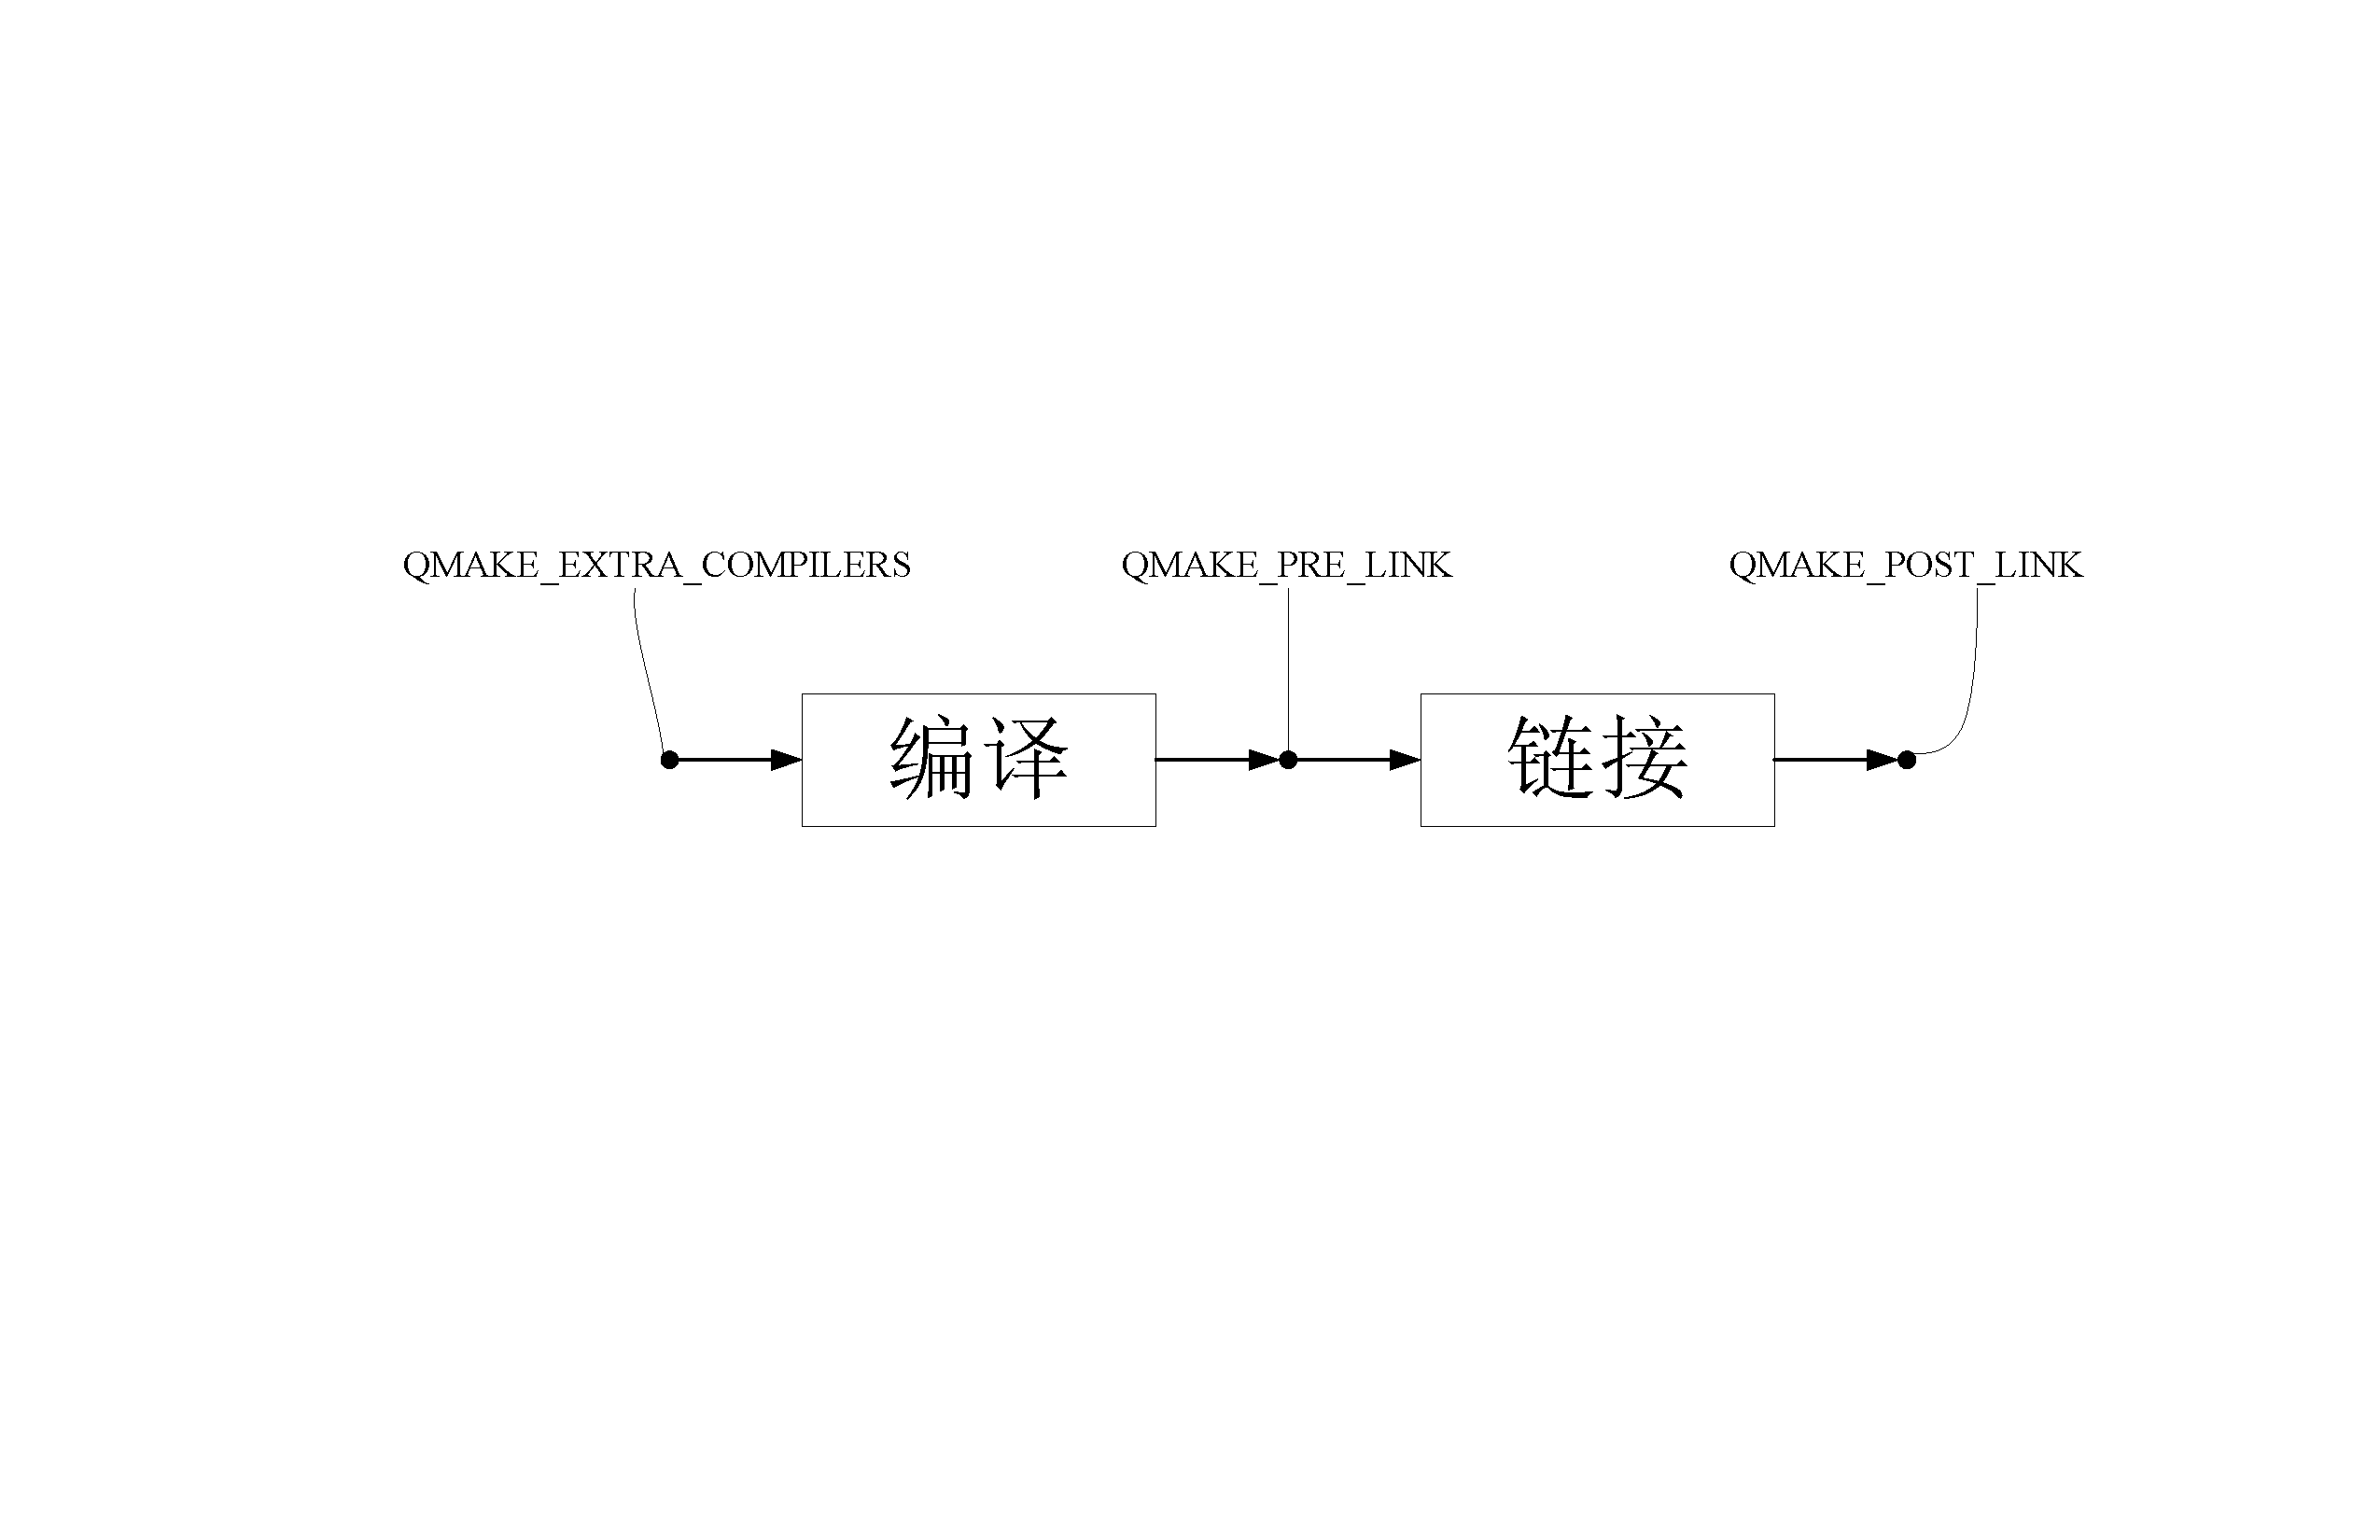
\includegraphics[width=0.95\textwidth]{chapter01/images/advance_use_qmake.pdf} %图片路径
\caption{qmake对C/C{\sourcefonttwo{}+}{\sourcefonttwo{}+}编译链接过程中的控制点} %标题
\label{p000002} %索引
\end{figure}
%end图片


如\figurename\ \ref{p000002}
一个C/C{\sourcefonttwo{}+}{\sourcefonttwo{}+}程序编译至少可以抽象出三个节点,
源代码编译前,
链接前以及链接后。
这三个时刻分别对应于qmake变量:
QMAKE\underline{\hspace{0.5em}}EXTRA\underline{\hspace{0.5em}}COMPILERS,
QMAKE\underline{\hspace{0.5em}}PRE\underline{\hspace{0.5em}}LINK以及
QMAKE\underline{\hspace{0.5em}}POST\underline{\hspace{0.5em}}LINK。

使用这三个控制变量,用户可以在这三个时刻执行自定义命令。

本节代码树
如\treeindexnumbernameone\ \ref{d000000}
所示,
“advance\underline{\hspace{0.5em}}use\underline{\hspace{0.5em}}qmake.pro”文件
如\filesourcenumbernameone\ \ref{f000004}
所示。

%\begin{spacing}{1.0}
%\FloatBarrier
\refstepcounter{treeindexnumber}\label{d000000}    %增加目录树编号
\begin{thebookfilesourceonepathtree}[escapeinside={(*@}{@*)},
caption=GoodLuck,
numbers=none,
title=\treeindexnumbernameone \thetreeindexnumber
]
.
├── advance_use_qmake.pro
├── after_run
│   ├── after_run.pro
│   └── main.cpp
├── before_run
│   ├── before_run.pro
│   └── main.cpp
├── new_moc
│   ├── main.cpp
│   └── new_moc.pro
└── the_run
    ├── main.cpp
    ├── test1.hpp
    ├── test2.hpp
    └── the_run.pro(*@\marginpar[\hfill\setlength\fboxsep{2pt}\fbox{\footnotesize{\kaishu\parbox{1em}{\setlength{\baselineskip}{2pt}\treeindexnumbernameone}}\footnotesize{\thetreeindexnumber}}]{\setlength\fboxsep{2pt}\fbox{\footnotesize{\kaishu\parbox{1em}{\setlength{\baselineskip}{2pt}\treeindexnumbernameone}}\footnotesize{\thetreeindexnumber}}}@*)\end{thebookfilesourceonepathtree}          %抄录环境
\addtocounter{lstlisting}{-1}   %sub lstlisting counter ...
%\end{spacing}
 %tree.txt

%\begin{spacing}{1.0}
\refstepcounter{filesourcenumber}\label{f000004}    %增加源代码编号
\FloatBarrier                                  %强制完成浮动体布局
\begin{thebookfilesourceone}[escapeinside={(*@}{@*)},
caption=GoodLuck,
title=\filesourcenumbernameone \thefilesourcenumber
]
#advance_use_qmake.pro
TEMPLATE = subdirs

CONFIG += ordered

new_moc.file = $$PWD/new_moc/new_moc.pro
SUBDIRS += new_moc

before_run.file = $$PWD/before_run/before_run.pro
SUBDIRS += before_run

after_run.file = $$PWD/after_run/after_run.pro
SUBDIRS += after_run

the_run.file = $$PWD/the_run/the_run.pro
SUBDIRS += the_run(*@\marginpar[\hfill\setlength\fboxsep{2pt}\fbox{\footnotesize{\kaishu\parbox{1em}{\setlength{\baselineskip}{2pt}\filesourcenumbernameone}}\footnotesize{\thefilesourcenumber}}]{\setlength\fboxsep{2pt}\fbox{\footnotesize{\kaishu\parbox{1em}{\setlength{\baselineskip}{2pt}\filesourcenumbernameone}}\footnotesize{\thefilesourcenumber}}}@*)\end{thebookfilesourceone}          %抄录环境
\addtocounter{lstlisting}{-1}   %sub lstlisting counter ...
%\end{spacing}
 %advance_use_qmake.pro

本案例向读者展示:
\begin{enumerate}
\item 在编译开始前,qmake调用“程序new\underline{\hspace{0.5em}}moc”自动生成cpp文件并加入编译过程;
\item 在链接前qmake调用“程序before\underline{\hspace{0.5em}}run”,“程序before\underline{\hspace{0.5em}}run”
向“the\underline{\hspace{0.5em}}run文件夹”下建立一个“before\underline{\hspace{0.5em}}run.txt文件”;
\item 在链接完成后qmake调用“程序after\underline{\hspace{0.5em}}run”,“程序after\underline{\hspace{0.5em}}run”
向“the\underline{\hspace{0.5em}}run”文件夹下建立一个“after\underline{\hspace{0.5em}}run.txt文件”;
\end{enumerate}

主要分析一下“the\underline{\hspace{0.5em}}run.pro”
(如\filesourcenumbernameone\ \ref{f000005})。

%##########################################################

\begin{itemize}
\item 第28\raisebox{0.16ex}{\sourcefonttwo\~{}}41行展示了如何使用
“QMAKE\underline{\hspace{0.5em}}EXTRA\underline{\hspace{0.5em}}COMPILERS”。

“QMAKE\underline{\hspace{0.5em}}EXTRA\underline{\hspace{0.5em}}COMPILERS”往往用于自定义一种“编译时编译”规则,
实际上Qt的moc就是这么实现的。
读者可以用此技术实现自定义代码生成器,
不过这需要读者有编译原理相关知识。
\item 第44\raisebox{0.16ex}{\sourcefonttwo\~{}}49行展示了如何使用
“QMAKE\underline{\hspace{0.5em}}PRE\underline{\hspace{0.5em}}LINK”。

实际上,对于一般用户,
“QMAKE\underline{\hspace{0.5em}}PRE\underline{\hspace{0.5em}}LINK”并不常用。
除非读者要实现类似
将其它编译器编译的二进制文件加入本次编译过程的功能。
\item 第52\raisebox{0.16ex}{\sourcefonttwo\~{}}57行展示了如何使用
“QMAKE\underline{\hspace{0.5em}}POST\underline{\hspace{0.5em}}LINK”。

“QMAKE\underline{\hspace{0.5em}}POST\underline{\hspace{0.5em}}LINK”往往用来
自定义“make install”。虽然qmake有默认的“make install”规则。
不过,本书并不准备介绍。因为,
一个实际应用程序的“make install”往往不是简单的拷贝,
而是需要对文件进行加密、压缩或者对文件进行语法检查等额外的任务。
而利用C{\sourcefonttwo{}+}{\sourcefonttwo{}+} 17的filesystem模块自己实现一个单纯的拷贝程序并不复杂。
因而,本书介绍更加通用的“QMAKE\underline{\hspace{0.5em}}POST\underline{\hspace{0.5em}}LINK”,
而不介绍qmake的专用语法。
\end{itemize}

%##########################################################


%\begin{spacing}{1.0}
\refstepcounter{filesourcenumber}\label{f000005}    %增加源代码编号
\FloatBarrier                                  %强制完成浮动体布局
\begin{thebookfilesourceone}[escapeinside={(*@}{@*)},
caption=GoodLuck,
title=\filesourcenumbernameone \thefilesourcenumber
]
#the_run.pro
QT -= gui
QT -= core

CONFIG += console

CONFIG(debug,debug|release){
    TARGET = the_run_debug
}else{
    TARGET = the_run
}

TEMPLATE = app

win32-msvc*{
    QMAKE_CXXFLAGS += /std:c++latest
}else{
    CONFIG += c++17
    LIBS += -lstdc++fs
}

SOURCES += $$PWD/main.cpp
DESTDIR =  $$PWD/../bin

DEFINES += QT_DEPRECATED_WARNINGS

#when before build new_moc will call ...
new_moc.dependency_type = TYPE_C
new_moc.variable_out =    SOURCES
new_moc.output  = moc_new_${QMAKE_FILE_BASE}.cpp
CONFIG(debug,debug|release){
    new_moc.commands = \
$${DESTDIR}/new_moc_debug ${QMAKE_FILE_NAME} ${QMAKE_FILE_OUT}
}else{
    new_moc.commands = \
$${DESTDIR}/new_moc ${QMAKE_FILE_NAME} ${QMAKE_FILE_OUT}
}
NEW_MOC_HEADERS = test2.hpp test1.hpp
new_moc.input = NEW_MOC_HEADERS
QMAKE_EXTRA_COMPILERS += new_moc
export(QMAKE_EXTRA_COMPILERS)

#when link started before_run will call ...
CONFIG(debug,debug|release){
    QMAKE_PRE_LINK += $${DESTDIR}/before_run_debug $$PWD
}else{
    QMAKE_PRE_LINK += $${DESTDIR}/before_run $$PWD
}
export(QMAKE_PRE_LINK)

#when link finished after_run will call ...
CONFIG(debug,debug|release){
    QMAKE_POST_LINK += $${DESTDIR}/after_run_debug $$PWD
}else{
    QMAKE_POST_LINK += $${DESTDIR}/after_run $$PWD
}
export(QMAKE_POST_LINK)(*@\marginpar[\hfill\setlength\fboxsep{2pt}\fbox{\footnotesize{\kaishu\parbox{1em}{\setlength{\baselineskip}{2pt}\filesourcenumbernameone}}\footnotesize{\thefilesourcenumber}}]{\setlength\fboxsep{2pt}\fbox{\footnotesize{\kaishu\parbox{1em}{\setlength{\baselineskip}{2pt}\filesourcenumbernameone}}\footnotesize{\thefilesourcenumber}}}@*)\end{thebookfilesourceone}          %抄录环境
\addtocounter{lstlisting}{-1}   %sub lstlisting counter ...
%\end{spacing}
 %the_run.pro



其余的,
“before\underline{\hspace{0.5em}}run.pro”
(如\filesourcenumbernameone\ \ref{f000008})
、“before\underline{\hspace{0.5em}}run/main.cpp”
(如\filesourcenumbernameone\ \ref{f000009})
、“after\underline{\hspace{0.5em}}run.pro”
(如\filesourcenumbernameone\ \ref{f000006})
、“after\underline{\hspace{0.5em}}run/main.cpp”
(如\filesourcenumbernameone\ \ref{f000007})
、“new\underline{\hspace{0.5em}}moc.pro”
(如\filesourcenumbernameone\ \ref{f00000b})
、“new\underline{\hspace{0.5em}}moc/main.cpp”
(如\filesourcenumbernameone\ \ref{f00000c})
和
“the\underline{\hspace{0.5em}}run/main.cpp”
(如\filesourcenumbernameone\ \ref{f00000a})
没有新知识点,本书不赘述。

%\begin{spacing}{1.0}
\refstepcounter{filesourcenumber}\label{f000008}    %增加源代码编号
\FloatBarrier                                  %强制完成浮动体布局
\begin{thebookfilesourceone}[escapeinside={(*@}{@*)},
caption=GoodLuck,
title=\filesourcenumbernameone \thefilesourcenumber
]
#before_run.pro
QT -= gui
QT -= core

CONFIG += console

CONFIG(debug,debug|release){
    TARGET = before_run_debug
}else{
    TARGET = before_run
}

TEMPLATE = app

win32-msvc*{
    QMAKE_CXXFLAGS += /std:c++latest
}else{
    CONFIG += c++17
    LIBS += -lstdc++fs
}

SOURCES += $$PWD/main.cpp
DESTDIR =  $$PWD/../bin

DEFINES += QT_DEPRECATED_WARNINGS(*@\marginpar[\hfill\setlength\fboxsep{2pt}\fbox{\footnotesize{\kaishu\parbox{1em}{\setlength{\baselineskip}{2pt}\filesourcenumbernameone}}\footnotesize{\thefilesourcenumber}}]{\setlength\fboxsep{2pt}\fbox{\footnotesize{\kaishu\parbox{1em}{\setlength{\baselineskip}{2pt}\filesourcenumbernameone}}\footnotesize{\thefilesourcenumber}}}@*)\end{thebookfilesourceone}          %抄录环境
\addtocounter{lstlisting}{-1}   %sub lstlisting counter ...
%\end{spacing}
 %before_run.pro
%\begin{spacing}{1.0}
\refstepcounter{filesourcenumber}\label{f000009}    %增加源代码编号
\FloatBarrier                                  %强制完成浮动体布局
\begin{thebookfilesourceone}[escapeinside={(*@}{@*)},
caption=GoodLuck,
title=\filesourcenumbernameone \thefilesourcenumber
]
/*main.cpp*/
#if __has_include(<filesystem>)
#include <filesystem>
namespace fs = std::filesystem;
#else
#include <experimental/filesystem>
namespace fs = std::experimental::filesystem;
#endif

#include <iostream>
#include <fstream>
#include <chrono>

class OStream final : public std::ofstream {
    using Super = std::ofstream;
public:
    template<typename T,
        typename = std::enable_if_t<
        std::is_constructible_v<Super, T && > > >
        inline OStream(T && arg) :
        Super(std::forward<T>(arg)) {
    }
    template<typename T,
        typename = void,
        typename = std::enable_if_t<
        !std::is_constructible_v<Super, T && > > >
        inline OStream(T && arg) :
        Super(std::forward<T>(arg).string()) {
    }
};

/* 在特定文件夹下建立一个before_run.txt
 * 并输出程序运行时时间戳 */
int main(int argc, char ** argv) {
    std::cout << "before_run : "
        << argc << std::endl;
    if (argc < 2) {
        return -1;
    }
    fs::path varPath{ argv[1] };
    OStream stream{ varPath / "before_run.txt" };
    stream << std::chrono::
        high_resolution_clock::now()
        .time_since_epoch().count();
    stream << std::endl;
    return 0;
}(*@\marginpar[\hfill\setlength\fboxsep{2pt}\fbox{\footnotesize{\kaishu\parbox{1em}{\setlength{\baselineskip}{2pt}\filesourcenumbernameone}}\footnotesize{\thefilesourcenumber}}]{\setlength\fboxsep{2pt}\fbox{\footnotesize{\kaishu\parbox{1em}{\setlength{\baselineskip}{2pt}\filesourcenumbernameone}}\footnotesize{\thefilesourcenumber}}}@*)\end{thebookfilesourceone}          %抄录环境
\addtocounter{lstlisting}{-1}   %sub lstlisting counter ...
%\end{spacing}
 %before_run/main.cpp

%\begin{spacing}{1.0}
\refstepcounter{filesourcenumber}\label{f000006}    %增加源代码编号
\FloatBarrier                                  %强制完成浮动体布局
\begin{thebookfilesourceone}[escapeinside={(*@}{@*)},
caption=GoodLuck,
title=\filesourcenumbernameone \thefilesourcenumber
]
#after_run.pro
QT -= gui
QT -= core

CONFIG += console

CONFIG(debug,debug|release){
    TARGET = after_run_debug
}else{
    TARGET = after_run
}

TEMPLATE = app

win32-msvc*{
    QMAKE_CXXFLAGS += /std:c++latest
}else{
    CONFIG += c++17
    LIBS += -lstdc++fs
}

SOURCES += $$PWD/main.cpp
DESTDIR =  $$PWD/../bin

DEFINES += QT_DEPRECATED_WARNINGS(*@\marginpar[\hfill\setlength\fboxsep{2pt}\fbox{\footnotesize{\kaishu\parbox{1em}{\setlength{\baselineskip}{2pt}\filesourcenumbernameone}}\footnotesize{\thefilesourcenumber}}]{\setlength\fboxsep{2pt}\fbox{\footnotesize{\kaishu\parbox{1em}{\setlength{\baselineskip}{2pt}\filesourcenumbernameone}}\footnotesize{\thefilesourcenumber}}}@*)\end{thebookfilesourceone}          %抄录环境
\addtocounter{lstlisting}{-1}   %sub lstlisting counter ...
%\end{spacing}
 %after_run.pro
%\begin{spacing}{1.0}
\refstepcounter{filesourcenumber}\label{f000007}    %增加源代码编号
\FloatBarrier                                  %强制完成浮动体布局
\begin{thebookfilesourceone}[escapeinside={(*@}{@*)},
caption=GoodLuck,
title=\filesourcenumbernameone \thefilesourcenumber
]
/*main.cpp*/
#if __has_include(<filesystem>)
#include <filesystem>
namespace fs = std::filesystem;
#else
#include <experimental/filesystem>
namespace fs = std::experimental::filesystem;
#endif

#include <iostream>
#include <fstream>
#include <chrono>

class OStream final : public std::ofstream {
    using Super = std::ofstream;
public:
    template<typename T,
        typename = std::enable_if_t<
        std::is_constructible_v<Super, T && > > >
        inline OStream(T && arg) :
        Super(std::forward<T>(arg)) {
    }
    template<typename T,
        typename = void,
        typename = std::enable_if_t<
        !std::is_constructible_v<Super, T && > > >
        inline OStream(T && arg) :
        Super(std::forward<T>(arg).string()) {
    }
};

/* 在特定文件夹下建立一个after_run.txt
 * 并输出程序运行时时间戳 */
int main(int argc, char ** argv) {
    std::cout << "after_run : "
        << argc << std::endl;
    if (argc < 2) {
        return -1;
    }
    fs::path varPath{ argv[1] };
    OStream stream{ varPath / "after_run.txt" };
    stream << std::chrono::
        high_resolution_clock::now()
        .time_since_epoch().count();
    stream << std::endl;
    return 0;
}(*@\marginpar[\hfill\setlength\fboxsep{2pt}\fbox{\footnotesize{\kaishu\parbox{1em}{\setlength{\baselineskip}{2pt}\filesourcenumbernameone}}\footnotesize{\thefilesourcenumber}}]{\setlength\fboxsep{2pt}\fbox{\footnotesize{\kaishu\parbox{1em}{\setlength{\baselineskip}{2pt}\filesourcenumbernameone}}\footnotesize{\thefilesourcenumber}}}@*)\end{thebookfilesourceone}          %抄录环境
\addtocounter{lstlisting}{-1}   %sub lstlisting counter ...
%\end{spacing}
 %after_run/main.cpp

%\begin{spacing}{1.0}
\refstepcounter{filesourcenumber}\label{f00000b}    %增加源代码编号
\FloatBarrier                                  %强制完成浮动体布局
\begin{thebookfilesourceone}[escapeinside={(*@}{@*)},
caption=GoodLuck,
title=\filesourcenumbernameone \thefilesourcenumber
]
#new_moc.pro
QT -= gui
QT -= core

CONFIG += console

CONFIG(debug,debug|release){
    TARGET = new_moc_debug
}else{
    TARGET = new_moc
}

TEMPLATE = app

win32-msvc*{
    QMAKE_CXXFLAGS += /std:c++latest
}else{
    CONFIG += c++17
    LIBS += -lstdc++fs
}

SOURCES += $$PWD/main.cpp
DESTDIR =  $$PWD/../bin

DEFINES += QT_DEPRECATED_WARNINGS(*@\marginpar[\hfill\setlength\fboxsep{2pt}\fbox{\footnotesize{\kaishu\parbox{1em}{\setlength{\baselineskip}{2pt}\filesourcenumbernameone}}\footnotesize{\thefilesourcenumber}}]{\setlength\fboxsep{2pt}\fbox{\footnotesize{\kaishu\parbox{1em}{\setlength{\baselineskip}{2pt}\filesourcenumbernameone}}\footnotesize{\thefilesourcenumber}}}@*)\end{thebookfilesourceone}          %抄录环境
\addtocounter{lstlisting}{-1}   %sub lstlisting counter ...
%\end{spacing}
 %new_moc.pro
%\begin{spacing}{1.0}
\refstepcounter{filesourcenumber}\label{f00000c}    %增加源代码编号
\FloatBarrier                                  %强制完成浮动体布局
\begin{thebookfilesourceone}[escapeinside={(*@}{@*)},
caption=GoodLuck,
title=\filesourcenumbernameone \thefilesourcenumber
]
/*main.cpp*/
#include <iostream>
#include <fstream>

#if __has_include(<filesystem>)
#include <filesystem>
namespace fs = std::filesystem;
#else
#include <experimental/filesystem>
namespace fs = std::experimental::filesystem;
#endif

/*生成一个用于测试的.cpp,用于在控制台输出“Good Luck!”*/
int main(int argc, char ** argv) {
    std::cout << "new_moc : "
        << argc << std::endl;
    if (argc < 3) {
        return -1;
    }
    std::ifstream varInput{ argv[1] };
    std::ofstream varOutput{ argv[2] };
    varOutput << "/*****************************/";
    varOutput << std::endl;
    varOutput << "#include \"";
    varOutput << argv[1];
    varOutput << "\"";
    varOutput << std::endl;
    varOutput << u8R"(inline static int a = [](){
               std::cout << "Good Luck!" <<std::endl;
               return 12;
               }() ; )";
    varOutput << std::endl;
    return 0;
}(*@\marginpar[\hfill\setlength\fboxsep{2pt}\fbox{\footnotesize{\kaishu\parbox{1em}{\setlength{\baselineskip}{2pt}\filesourcenumbernameone}}\footnotesize{\thefilesourcenumber}}]{\setlength\fboxsep{2pt}\fbox{\footnotesize{\kaishu\parbox{1em}{\setlength{\baselineskip}{2pt}\filesourcenumbernameone}}\footnotesize{\thefilesourcenumber}}}@*)\end{thebookfilesourceone}          %抄录环境
\addtocounter{lstlisting}{-1}   %sub lstlisting counter ...
%\end{spacing}
 %new_moc/main.cpp

%\begin{spacing}{1.0}
\refstepcounter{filesourcenumber}\label{f00000a}    %增加源代码编号
\FloatBarrier                                  %强制完成浮动体布局
\begin{thebookfilesourceone}[escapeinside={(*@}{@*)},
caption=GoodLuck,
title=\filesourcenumbernameone \thefilesourcenumber
]
/*main.cpp*/
#if __has_include(<filesystem>)
#include <filesystem>
namespace fs = std::filesystem;
#else
#include <experimental/filesystem>
namespace fs = std::experimental::filesystem;
#endif
#include <iostream>

int main(int, char **) {
    std::cout << "the_run" << std::endl;
    return 0;
}(*@\marginpar[\hfill\setlength\fboxsep{2pt}\fbox{\footnotesize{\kaishu\parbox{1em}{\setlength{\baselineskip}{2pt}\filesourcenumbernameone}}\footnotesize{\thefilesourcenumber}}]{\setlength\fboxsep{2pt}\fbox{\footnotesize{\kaishu\parbox{1em}{\setlength{\baselineskip}{2pt}\filesourcenumbernameone}}\footnotesize{\thefilesourcenumber}}}@*)\end{thebookfilesourceone}          %抄录环境
\addtocounter{lstlisting}{-1}   %sub lstlisting counter ...
%\end{spacing}
 %the_run/main.cpp


%%%%%%%%%%%%%%%%%%%%%%%%%%%%%%%%%%%%%%%%%%%%%%%%%%%%%%%%
\FloatBarrier
\subsection{
qmake生成Visual Studio工程
}\label{ss000910}

使用qmake生成Visual Studio工程十分简单,
其核心指令只有一条,
如\commandnumbernameone\ \ref{command000003}:

%\begin{spacing}{1.0}
%\FloatBarrier
\refstepcounter{commandnumber}\label{command000003}    %增加命令行编号
\begin{thebookfilesourceonecommand}[escapeinside={(*@}{@*)},
caption=GoodLuck,
title=\commandnumbernameone \thecommandnumber
]
qmake -r -tp vc < 工程名称 >(*@\marginpar[\hfill\setlength\fboxsep{2pt}\fbox{\footnotesize{\kaishu\parbox{1em}{\setlength{\baselineskip}{2pt}\commandnumbernameone}}\footnotesize{\thecommandnumber}}]{\setlength\fboxsep{2pt}\fbox{\footnotesize{\kaishu\parbox{1em}{\setlength{\baselineskip}{2pt}\commandnumbernameone}}\footnotesize{\thecommandnumber}}}@*)\end{thebookfilesourceonecommand}          %抄录环境
\addtocounter{lstlisting}{-1}   %sub lstlisting counter ...
%\end{spacing}


在Windows平台下读者如果想在命令行下运行此命令需要设置
好运行环境。


读者可以在Qt安装目录下找到“qtenv2.bat”文件。其中一个合法路径是:
\begin{littlelongworld}
C:\textbackslash{}Qt\textbackslash{}Qt5.12.0\textbackslash{}5.12.0\textbackslash{}msvc2017\underline{\hspace{0.5em}}64\textbackslash{}bin\textbackslash{}qtenv2.bat
\end{littlelongworld}
\hspace*{\parindent}读者要修改“qtenv2.bat”文件。
32位开发环境将“vcvarsall.bat”或
64位开发环境将“vcvar64.bat”引入并执行。

如\filesourcenumbernameone\ \ref{f000017}
第5行所示:
%\begin{spacing}{1.0}
\refstepcounter{filesourcenumber}\label{f000017}    %增加源代码编号
\FloatBarrier                                  %强制完成浮动体布局
\begin{thebookfilesourceone}[escapeinside={(*@}{@*)},
caption=GoodLuck,
title=\filesourcenumbernameone \thefilesourcenumber
]
@echo off
echo Setting up environment for Qt usage...
set PATH=C:\Qt1\5.12.0\msvc2017_64\bin;%PATH%
cd /D C:\Qt1\5.12.0\msvc2017_64
call "C:/Program Files (x86)/Microsoft Visual Studio/2017/Enterprise/VC/Auxiliary/Build/vcvars64.bat"
echo Remember to call vcvarsall.bat to complete environment setup!(*@\marginpar[\hfill\setlength\fboxsep{2pt}\fbox{\footnotesize{\kaishu\parbox{1em}{\setlength{\baselineskip}{2pt}\filesourcenumbernameone}}\footnotesize{\thefilesourcenumber}}]{\setlength\fboxsep{2pt}\fbox{\footnotesize{\kaishu\parbox{1em}{\setlength{\baselineskip}{2pt}\filesourcenumbernameone}}\footnotesize{\thefilesourcenumber}}}@*)\end{thebookfilesourceone}          %抄录环境
\addtocounter{lstlisting}{-1}   %sub lstlisting counter ...
%\end{spacing}
 %qtenv2.windows.bat.txt

以后读者在Windows平台下运行“qtenv2.bat”就
可以得到一个完整的运行环境了。

\FloatBarrier
\subsection{
获得更多qmake帮助
}\label{ss000a10}


本书所介绍的知识已经足够帮助读者搭建绝大多数
大型复杂应用程序。
但软件项目如此复杂,
读者可能需要更进一步的知识才能解决手头的问题。

Qt的帮助系统一向被认为是各个软件项目中最好的之一。
读者只需要打开Qt Creator,
在帮助的索引搜索栏里面输入“qmake”,一切读者需要的信息就出现了。

\begin{itemize}

\item qmake的所有控制变量

要获得qmake的所有控制变量帮助信息,只需要单击
“qmake Variable Reference”即可,
如\figurename\ \ref{p000003}。

%begin图片
\begin{figure}[htb] %浮动体 here and top ...
%there must use marginnote ...
\marginnote{\setlength\fboxsep{2pt}\fbox{\footnotesize{\kaishu\figurename\,}\footnotesize{\ref{p000003}}}}\centering %中心对齐
\setlength\fboxsep{0pt}\fcolorbox[rgb]{0,0,0}{0.97,0.98,0.99}{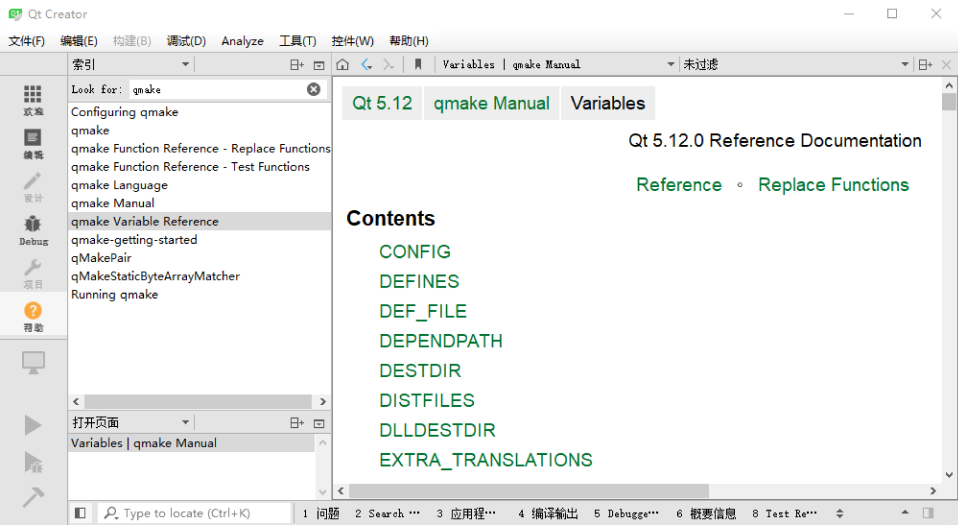
\includegraphics[width=0.95\textwidth]{the_book_image/p000003.pdf}} %图片路径
\caption{qmake Variable Reference} %标题
\label{p000003} %索引
\end{figure}
%end图片


\item qmake控制台运行参数

要获得qmake的所有控制台运行参数相关信息,只需要单击
“Running qmake”即可,
如\figurename\ \ref{p000004}。
%begin图片
\begin{figure}[htb] %浮动体 here and top ...
%there must use marginnote ...
\marginnote{\setlength\fboxsep{2pt}\fbox{\footnotesize{\kaishu\figurename\,}\footnotesize{\ref{p000004}}}}\centering %中心对齐
\setlength\fboxsep{0pt}\fcolorbox[rgb]{0,0,0}{0.97,0.98,0.99}{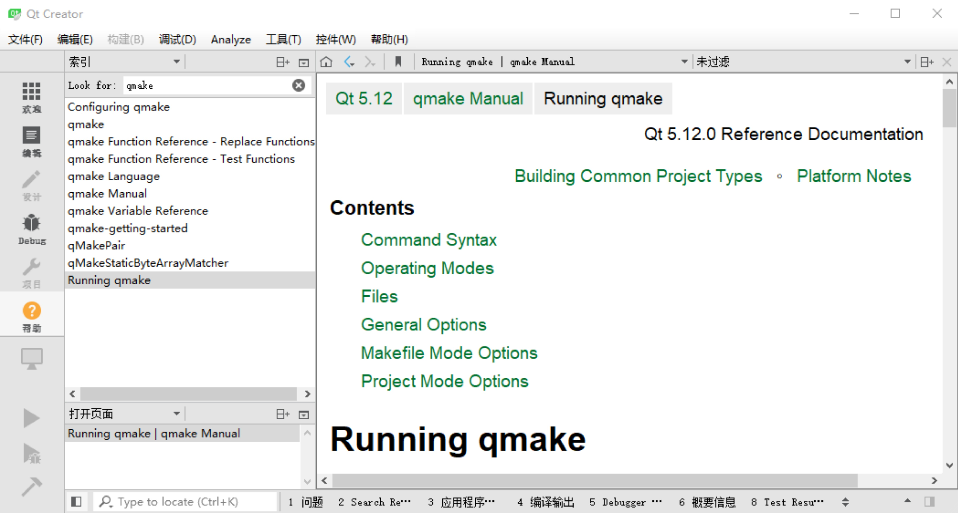
\includegraphics[width=0.95\textwidth]{the_book_image/p000004.pdf}} %图片路径
\caption{Running qmake} %标题
\label{p000004} %索引
\end{figure}
%end图片


\item qmake的完整语法

要完整的了解qmake的所有语法,只需要单击
“qmake Language”即可,
如\figurename\ \ref{p000005}。
%begin图片
\begin{figure}[htb] %浮动体 here and top ...
%there must use marginnote ...
\marginnote{\setlength\fboxsep{2pt}\fbox{\footnotesize{\kaishu\figurename\,}\footnotesize{\ref{p000005}}}}\centering %中心对齐
\setlength\fboxsep{0pt}\fcolorbox[rgb]{0,0,0}{0.97,0.98,0.99}{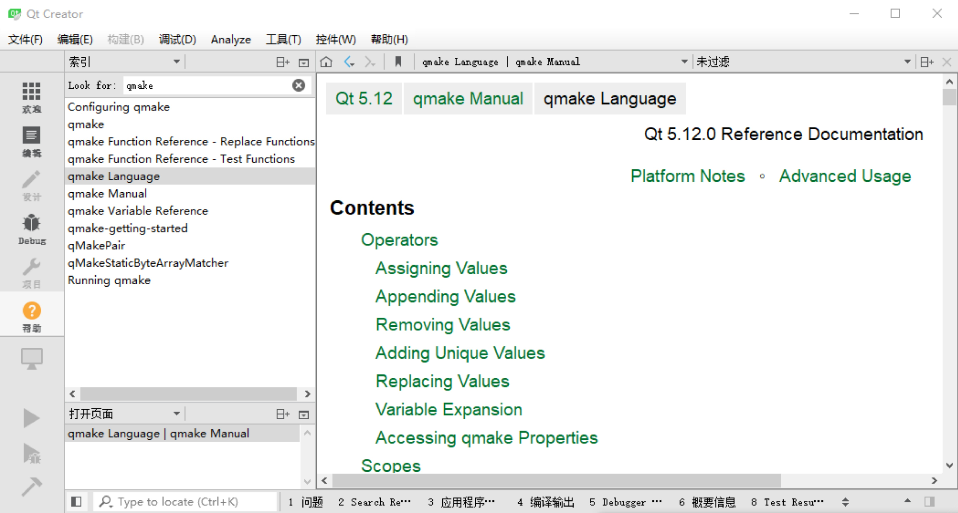
\includegraphics[width=0.95\textwidth]{the_book_image/p000005.pdf}} %图片路径
\caption{qmake Language} %标题
\label{p000005} %索引
\end{figure}
%end图片


\end{itemize}
















%使用XeLaTeX编译
%版权所有,翻版必究
%本文件由程序自动生成,任何修改将被覆盖
%2019 年 01 月 23 日



